\chapter{Diseño de la solución}
\label{chap:diseño}

En este capitulo describiremos la estrategia que seguimos para refactorizar el bucle MAPE-K \foreign{english}{Lite}. Como comentamos en la introducción, nuestro objetivo es adaptarlo a entornos \foreign{english}{cloud}. Esto implica transformarlo de un servicio monolítico a un sistema distribuido basado en microservicios. Se trata de un cambio arquitectónico importante. Por ello, queremos diseñar una estrategia ingenieril, teniendo en cuenta las particularidades del sistema.

Comenzaremos justificando la elección de este estilo arquitectónico y describiendo los beneficios que esperabamos obtener. A continuación detallaremos nuestro diseño. Definiremos los componentes que conforman nuestra arquitectura y describiremos cómo se distribuyó la funcionalidad del bucle como microservicios. Después, presentaremos cómo las conectamos. Mediante un estudio de los mecanismos de comunicación más populares, \textcolor{red}{elegimos los que más se ajustaban a cada escenario}. Finalmente, presentaremos la estructura final de nuestra arquitectura.

\section{¿Por qué usar microservicios?}

Una de las primeras decisiones que tomamos para el desarrollo de este trabajo fue elegir el estilo arquitectónico a emplear. Dado que queremos adaptar el bucle de control a entornos en la nube, será imprescindible que el estilo elegido esté preparado para ellos. Optamos por las \textbf{arquitecturas basadas en microservicios} por que son uno de los pilares de las aplicaciones \foreign{english}{cloud native}. \cite{gannonCloudNativeApplications2017} Gracias a este estilo, obteníamos una serie de beneficios que consideramos vitales para extender el bucle MAPE-K.

El más evidente fue poder \textbf{independizar la implementación} de los servicios. Si fuera necesario, podríamos emplear distintas tecnologías para cada uno. Aquellas que se ajusten más a la funcionalidad de estos. Incluso, podríamos ofrecer implementaciones alternativas de algunos componentes. Estos podrían ofrecer distintas estrategias de la misma funcionalidad: distintos planificadores, módulos de análisis, etc.

También vimos muy interesante el desarrollar \textbf{servicios \foreign{english}{plug \& play}}. Esto nos permitiría desplegar o eliminar componentes que modifiquen las capacidades de adaptación en tiempo real. Sin necesidad de parar el sistema en ningún momento. Por ejemplo, se podría desplegar un nuevo conjunto de reglas de adaptación que doten de capacidades de balanceo de carga al bucle de control.

Por otro lado, facilitaría \textbf{escalar la capacidad computacional} de cada servicio de forma independiente. Si por ejemplo un servicio concreto estuviera recibiendo más peticiones que los demás, no sería necesario instanciar el bucle completo. En su lugar, podemos limitarnos a desplegar una nueva instancia del componente afectado.

Finalmente, nos ayudaría a desacoplar el bucle de los componentes específicos para gestionar una solución autoadaptativa determinada. Así, en un futuro, podríamos aprovechar la misma infraestructura para manejar varias soluciones simultáneamente. Esto se conoce como multicliente o \textbf{\foreign{english}{multi-tennancy}}. \cite{aljahdaliMultitenancyCloudComputing2014} Como tiene importantes implicaciones a nivel de seguridad y gestión de los datos de los distintos clientes, en este trabajo no profundizaremos en esta rama.

Optar por un estilo arquitectónico determinado no sale gratis. Conlleva también una serie de desventajas que no pueden ignorarse. Aun así, se consideró que los beneficios las compensaban. Entre ellas, la más importante es un \textbf{aumento en la complejidad} del sistema. \cite{newmanBuildingMicroservicesDesigning2021} Pasamos de contar con un solo servicio monolítico a contar con varios más pequeños. Además, como se trata de un proceso lineal (monitor-analizador-planificador-ejecutor), cuantos más componentes tengamos, mayor número de puntos de fallo tendremos.

Esto impacta también en la operación del sistema. Necesitamos mantener operativos los servicios. Esto requerira de emplear

Por otro lado, al contar con más componentes, requiere de soluciones de monitorización y \foreign{english}{logging} más avanzadas. \cite{parkerProblemDistributedTracing2020} Una sola petición puede desencadenar llamadas a otros servicios. Sin una buena solución de \textbf{observabilidad} puede ser muy difícil analizar el impacto que tienen. Incluso para la depuración y detección de fallos.

\section{Distribución de los componentes}

Habiendo optado por una arquitectura basada en microservicios, el primer paso que tomamos fue identificar qué servicios la compondrían. Por suerte, partíamos de un sistema existente con una arquitectura bien definida y documentada. Conocíamos el rol de cada uno de sus elementos y sus requisitos. Nos quedaba entonces determinar cómo agrupar estos elementos en servicios. ¿Cómo definimos las fronteras entre cada uno de ellos? ¿Qué componentes debe abarcar cada microservicio?

Para ello, nos basaremos en unas pautas para dividir aplicaciones monolíticas. \cite{newmanBuildingMicroservicesDesigning2021} Los servicios que definamos deben presentar \textbf{alta cohesión} en su funcionalidad. Es decir, siempre que sea posible, debemos agrupar la funcionalidad relacionada. De esta forma, podremos reducir las comunicaciones necesarias entre servicios. Así, una de las primeras decisiones que tomamos fue \textbf{separar cada etapa del bucle en su propio servicio}. Entre ellas existe una división funcional bien definida y pueden operar con cierta independencia. El conocimiento también tendría su propio microservicio Esto nos reportaría varios beneficios.

Imagen que indica la primera división y luego la segunda.

El más evidente es que nos permitía \textbf{independizar la implementación} de cada etapa. Si fuera necesario, podríamos emplear distintas tecnologías para cada una. Incluso podríamos ofrecer implementaciones alternativas de algunos componentes. Estos podrían ofrecer distintas estrategias de la misma funcionalidad: planificadores, módulos de análisis, etc.

Por otro lado, también nos permitirá \textbf{escalar} la capacidad computacional de cada etapa de forma independiente. Si por ejemplo el servicio de análisis estuviera recibiendo más peticiones que las demás, no sería necesario instanciar el bucle completo. En su lugar, podemos limitarnos a desplegar una nueva instancia del componente afectado.

Otra posible división de servicios era la relacionada con la información del dominio. Actualmente, el bucle está muy acoplado al dominio de sus recursos manejados. Todo corre bajo el mismo proceso: el bucle, los monitores, sus reglas de adaptación y demás elementos específicos de la solución. Ese proceso solo podrá manejar aquellos sistemas cuyos módulos tenga cargados.

\textcolor{red}{Podremos cambiar los componentes en caliente. Por ejemplo si queremos desplegar nuevas reglas o monitores mientras el sistema está en marcha. Sin necesidad de downtime por parte del recurso manejado. o pudiendo convivir temporalmente ambas instancias hasta que se confirme el despliegue.}

Decidimos entonces desacoplarlos. Separar cada etapa del bucle MAPE-K de los elementos específicos de cada solución. Así, tendremos cada etapa como un microservicio agnóstico a una solución concreta; y por otro lado, estarán los servicios específicos para cada solución, con conocimiento del dominio del recurso manejado: monitores, reglas de adaptación, efectores\dots

En cuanto al despliegue, mantendremos el bucle a nivel de sistema, \cite{mendoncaGeneralityVsReusability2018} como funcionaba hasta ahora. Esto significa que se desplegará conjuntamente con los microservicios del recurso manejado. En la figura \ref{fig:mape-k-microservices} mostramos los microservicios que componen nuestra arquitectura.

\begin{figure}[htb]
  \centering
  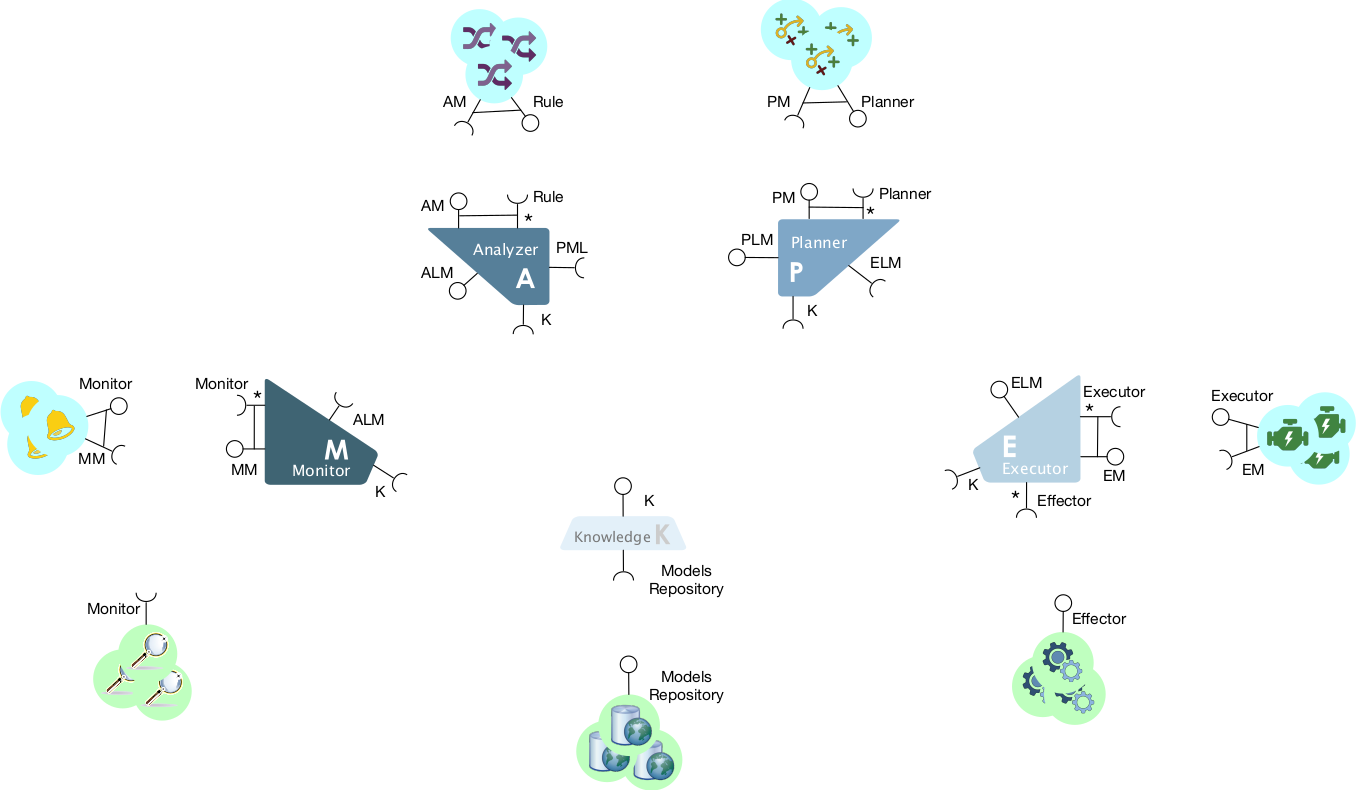
\includegraphics[scale=0.25]{cap_diseño/images/mape-k-microservices}
  \caption{Diagrama con los componentes que forman nuestra arquitectura distribuida}
  \label{fig:mape-k-microservices}
\end{figure}

\textcolor{red}{Figura \ref{fig:mape-k-microservices}: Borrar los servicios específicos de planificador y ejecutor. Agrupar los servicios para poder aumentar zoom y hacerlo más legible. Añadir línea de divisón entre la capa del bucle y el dominio del recurso manejado. Eliminar la dependencia entre el monitor y el módulo de análisis. Borrar también los planificadores específicos y los ejeecutre especficios.d}

\section{Conectando los servicios}

El siguiente problema al que nos enfrentamos está relacionado con la comunicación: si dividimos estos componentes en microservicios, ¿cómo deberían comunicarse? Hay que tener en cuenta que estos pueden estar desplegados y replicados en distintas máquinas. No podemos asumir que están en el mismo \foreign{english}{host}.

Aprovechando la separación entre bucle de control y el dominio del recurso, investigamos arquitecturas existentes. Nos decantamos por \textbf{arquitecturas de servicios jerarquizados}. Queríamos explotar esta separación para mantener al bucle aislado del dominio de la solución. Dimos con el estilo arquitectónico C2 (\emph {components and connectors})\cite{taylorComponentMessagebasedArchitectural1996a, UCISoftwareArchitecture}, en el que nos hemos inspirado.

\subsection{Jerarquías de microservicios: Arquitectura C2 y arquitectura limpia}

Este estilo organiza sus componentes en jerarquías o capas: cada servicio se encuentra en un nivel determinado, según su nivel de abstracción respecto al entorno de ejecución. En las capas inferiores, se encuentran los servicios más externos, más ''acoplados''. Por ejemplo, aquellos servicios que requieran de acceder al sistema de ficheros, estarían en esta capa. Por otro lado, en las capas superiores se encuentran los servicios en niveles de abstracción superior, que dependen lo mínimo. \textcolor{red}{Buscar ejemplo representativo}

En cuanto a la comunicación, un componente solo debe contactar con sus vecinos inmediatos (en una capa superior o inferior). Esto evita que el servicio pueda contactar con otras capas, limitando su alcance y su conocimiento sobre el resto del sistema. Además, dentro de un mismo nivel no pueden contactar entre ellos. Según la dirección de la comunicación, se emplean mecanismos distintos (figura \ref{fig:C2-arch-example}):

\begin{itemize}
  \item \textbf{Peticiones} (\emph{requests}): Se trata de solicitudes a un servicio concreto para que ejecute una acción. Un componente se comunica directamente con un vecino en una capa superior. La petición viaja de ''abajo a arriba'' en cuanto al nivel de abstracción. Por ejemplo, una petición de un cliente a un servicio web podría estar en esta categoría.

  \item \textbf{Notificaciones}: Un componente de más arriba en la jerarquía (más interno) envía un mensaje hacia abajo, sin especificar un receptor. Todos los servicios que estén por debajo lo recibirán y decidirán si tratarlo o no. Esto evita que nuestro servicio se acople a aquellos más concretos. Se puede emplear para comunicar eventos de interés al resto de servicios. Un ejemplo sería notificar al resto de servicios sobre la creación de un nuevo usuario.
\end{itemize}

\begin{figure}[htb]
  \centering
  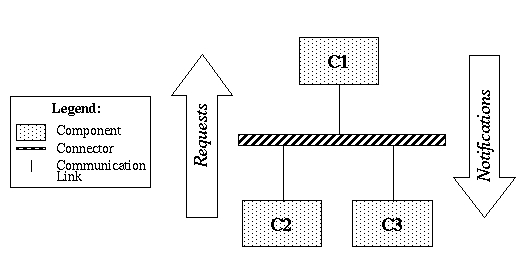
\includegraphics[scale=0.45]{cap_diseño/images/c2SampleArch}
  \caption[Ejemplo del estilo arquitectónico C2 (\emph{Components and Connectors})]{Ejemplo del estilo arquitectónico C2 (\emph{Components and Connectors}). \cite{UCISoftwareArchitecture}}
  \label{fig:C2-arch-example}
\end{figure}

Basándonos en este estilo, definimos las capas de nuestro sistema. Esto nos permitió organizar los microservicios en jerarquías, lo que nos ayudaría a definir las reglas de nuestra arquitectura. Distinguimos cuatro niveles, de menor a mayor nivel de abstracción:

\begin{itemize}
  \item \textbf{Nivel del recurso manejado}: En este nivel se encuentra el recurso manejado. Este implementa las sondas y efectores, los elementos que nos permiten interactuar con él. Hacen de intermediarios entre este y el resto del bucle, para reducir su acoplamiento.

  \item \textbf{Nivel de solución}: En esta capa se encuentran componentes del bucle específicos para una solución concreta: monitores, reglas de adaptación, etc. No los incluimos en el mismo nivel que las sondas y efectores porque están a un nivel de abstracción distinto. Estos elementos guardan dependencia con el propio bucle de control.

  \item \textbf{Nivel del bucle}: Aquí se encuentran los servicios de las etapas del bucle: servicio de monitorización, análisis, planificación y ejecución. Esta capa es agnóstica al dominio de los recursos manejados. Además, actúa como intermediario entre los servicios de la solución y el conocimiento. Limitan cómo se accede a él.

  \item \textbf{Conocimiento}: Es la capa más interna y la base de la arquitectura. No depende de ningún otro componente, por lo que tiene el mayor nivel de abstracción. Todos los componentes del nivel del bucle dependen de ella para funcionar.

\end{itemize}

Habiendo definido esta jerarquía, vimos ciertas similitudes con arquitecturas \foreign{english}{domain driven}, como \foreign{english}{Clean Architecture}. \cite{martinChapter22Clean2018a} En ella, el sistema se organiza en base a una \textbf{regla de dependencia}: <<\emph{la dependencia entre los componentes solo puede apuntar hacia dentro, hacia políticas de alto nivel}>>. Es decir, la arquitectura se organiza en \textbf{capas concéntricas}. En el centro se encuentra el dominio, con el mayor nivel de abstracción. Este no tiene dependencias con ninguna capa exterior. Por otro lado, cada capa más externa tiene dependencias sólo con la capa a la que envuelve. Sólo puede comunicarse con componentes dentro de esta.

Basándonos en la descripción anterior, optamos por representarla como una arquitectura \foreign{english}{knowledge driven} \cite{taylorSoftwareArchitectureFoundations2009}. Nuestra capa central será la del conocimiento. A partir de ahí, cada nivel superior dependería de aquella a la que ''envuelve'': el bucle al conocimiento, la solución al bucle\dots En la figura \ref{fig:clean-mapek-architecture} mostramos el resultado. Las flechas negras representan las peticiones, y las moradas, las notificaciones.

\begin{figure}[htb]
  \centering
  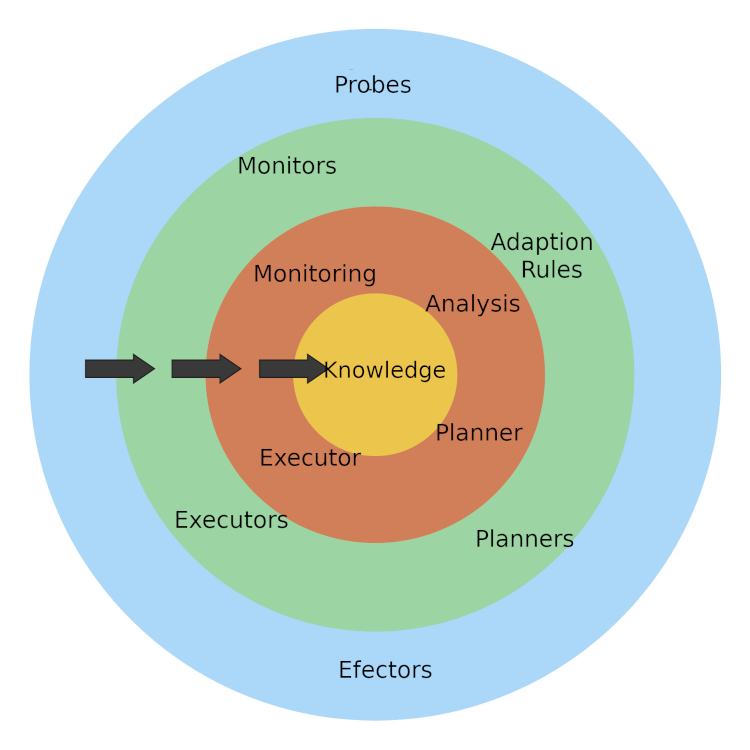
\includegraphics[scale=0.45]{cap_diseño/images/clean-arch-2-MAPEK-style-small}
  \caption[Representación de nuestra propuesta arquitectónica. Inspirado en Arquitectura Limpia (\emph{Clean Architecture}).]{Representación de nuestra propuesta arquitectónica. Inspirado en Arquitectura Limpia (\emph{Clean Architecture}). \footnotemark }
  \label{fig:clean-mapek-architecture}
\end{figure}

\footnotetext{Imagen original de arquitectura limpia obtenida de: \url{https://threedots.tech/post/ddd-cqrs-clean-architecture-combined/}}

\subsection{Definiendo los mecanismos de comunicación}

Como comentamos antes, nos inspiramos en los mecanismos de comunicación descritos por C2: las peticiones y notificaciones. Pero, durante nuestra etapa de prototipado, nos dimos cuenta que estos no cubren todas nuestras necesidades. Hay dos casos que no están contemplados: la comunicación del módulo de análisis con el planificador, y la del planificador con el ejecutor. Ambos módulos se encuentran en la misma capa. Y, como dependen del conocimiento para funcionar, no podíamos moverlos a una capa superior para emplear las notificaciones.

Requeríamos por tanto de un tercer patrón de comunicación. Detectamos que este conector debería ser dirigido: los mensajes van dirigidos a un componente determinado. Además, como los elementos están en el mismo nivel, no queremos que se acoplen entre ellos. Surgió entonces la idea de utilizar las peticiones asíncronas, una combinación de los dos patrones existentes. A continuación lo presentamos junto al resto de patrones de comunicaciones que empleamos:

\begin{itemize}
  \item \textbf{Peticiones síncronas}: Comunicaciones síncronas dirigidas a un servicio determinado. Un servicio contacta con otro con una petición o comando, y espera al resultado. Sólo están permitidas desde servicios de una capa más externa a un servicio en la capa interior adyacente.

  \item \textbf{Notificaciones}: Comunicaciones asíncronas no dirigidas. El servicio publica un evento que potencialmente recibirán todos los servicios en la capa externa adyacente. El cliente lo envía y continua su ejecución, sin esperar una respuesta.

  \item \textbf{Peticiones asíncronas}: Comunicaciones asíncronas dirigidas a un servicio determinado. Ideal para solicitar peticiones de trabajo asíncronas: se envían y el destinatario lo procesará cuando pueda. El cliente continuará su ejecución, sin esperar respuesta.

  Este mecanismo de comunicación solo está permitido entre elementos del mismo nivel. Para evitar el acoplamiento entre los componentes, deberemos buscar un conector que permita enviar el mensaje sin conocer específicamente al destinatario.

\end{itemize}

\subsection{Conectores}

Una vez determinadas las necesidades de comunicación de nuestro sistema, debemos buscar los conectores adecuados. Seguimos la estrategia descrita en \cite{taylorSoftwareArchitectureFoundations2009} para elegir conectores; y nos basamos en los patrones de comunicación en sistemas distribuidos descritos en \cite{newmanBuildingMicroservicesDesigning2021}.

La estrategia consiste en centrarse en las comunicaciones entre cada par de componentes, y a partir de sus requisitos, determinar el tipo de conector adecuado. Sabiendo que hemos optado por una arquitectura distribuida, la elección de los \textbf{tipos de conectores} se simplifica: los servicios pueden estar desplegados en máquinas distintas, por tanto el paso de mensajes será a través de la red.

Por ello, en lugar de recurrir a la taxonomía que lista \cite{mehtaTaxonomySoftwareConnectors2000}, optamos por consultar las estrategias de comunicación habituales para sistemas distribuidos descritas en \cite{newmanBuildingMicroservicesDesigning2021}. Se trata de cuatro mecanismos distintos: Invocación a métodos remotos (\foreign{english}{Remote Procedure Call}), APIs REST, consultas con GraphQL o \foreign{english}{brokers} de mensajería. Tuvimos que evaluarlos mediante un análisis de \foreign{english}{trade-offs} para determinar las ventajas y desventajas de cada uno.

\textcolor{red}{Hablar de smart endpoints, dumb pipes: \url{https://simplicable.com/new/smart-endpoints-and-dumb-pipes}}

\subsubsection{Tipos de conectores}

\textbf{Invocación de métodos remotos} o (\foreign{english}{\textbf{Remote Procedure Call}}): Este patrón se basa en el estilo cliente-servidor. Un servidor expone una serie de funciones que el cliente puede invocar mediante peticiones a través de la red. Estas peticiones incluyen el nombre de la función a ejecutar y sus parámetros. Al finalizar la ejecución, el servidor puede devolver un resultado, si lo hubiera. Existen varios protocolos que implementan este mecanismo como gRPC o SOAP.

En la programación orientada a objetos suele emplearse una evolución de RPC: el paradigma de \textbf{objetos distribuidos}. \cite{tanenbaumChapter10Distributed2007} En este caso, el programa cliente puede interactuar con objetos que se encuentran en servidores remotos como si fueran locales. Esta interacción se realiza a través de objetos que actúan como \foreign{english}{proxies}, abstrayendo de la llamada al servidor.

Los \foreign{english}{proxies} ofrecen una interfaz para que el cliente invoque sus métodos localmente. Por debajo, estos métodos realizan una llamada al servicio remoto donde se encuentra realmente. El servidor remoto procesa la petición y nos devolverá un resultado. En la figura \ref{fig:rpc-distributedobjects} tenemos un esquema de este mecanismo.

Los \foreign{english}{proxies} o (\foreign{english}{stubs} en la terminología de RPC) suelen generarse a partir de un contrato que define qué operaciones ofrecen los objetos. Por ejemplo: SOAP con WDSL, gRPC; o en el caso de objetos distribuidos, Java RMI.

\begin{figure}[htb]
  \centering
  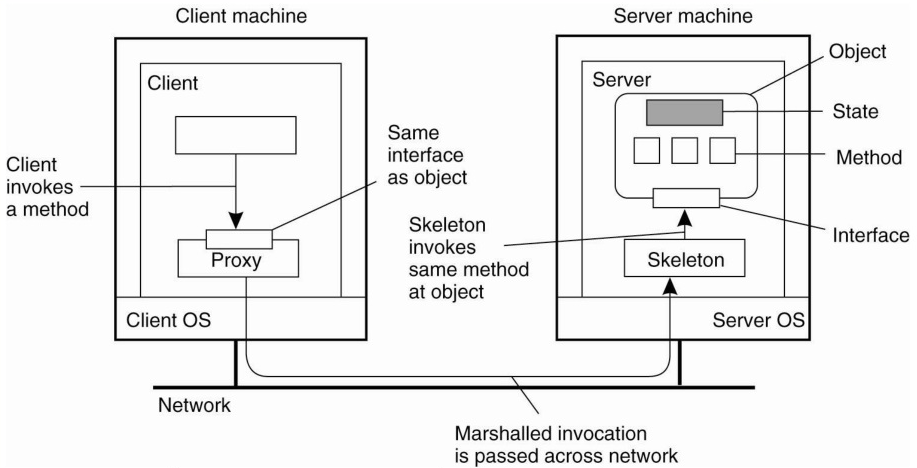
\includegraphics[scale=1.5]{cap_diseño/images/rpc-distributedobjects}
  \caption[Funcionamiento del sistema de objetos distribuidos.]{Funcionamiento del sistema de objetos distribuidos. Obtenido de \cite{tanenbaumChapter10Distributed2007}}
  \label{fig:rpc-distributedobjects}
\end{figure}

\begin{itemize}
  \item \textbf{Ventajas}:
  \begin{itemize}
    \item Permite distribuir la carga de procesamiento del sistema. Esto puede ayudar para escalar la aplicación.

    \item Abstrae al cliente de la interacción con un servidor remoto. Le resulta prácticamente indistinguible de un objeto local. Esto facilita la implementación.

  \end{itemize}

  \item \textbf{Desventajas}:
  \begin{itemize}
    \item \textbf{Dirigida}: Necesitamos conocer de antemano la ubicación del servidor al que queremos hacer una petición.

    \item Dificulta la integración con otras aplicaciones. Cada servicio ofrece sus propias funciones. No están estandarizadas.

    \item El cliente debe actualizarse y recompilarse con cada cambio en el esquema del servidor. Esto puede ser problemático para casos donde tenemos que desplegar una actualización para que nuestros clientes puedan continuar utilizando la aplicación.

    \item Respecto a los objetos distribuidos, no se puede abstraer completamente al cliente de las llamadas a través de la red. Pueden darse errores que no ocurrirían durante una invocación de un método sobre un objeto local. Por ejemplo, que el servidor no esté disponible. \cite{jausovecFallaciesDistributedSystems2020}

    \item \textcolor{red}{Si adoptamos sistemas como Java RMI, nuestro sistema se acopla a esa tecnología concreta. \cite{newmanBuildingMicroservicesDesigning2021}. Nos quita flexibilidad en cuanto a qué otras tecnologías podemos emplear en nuestra arquitectura.} ¿A Java o a Java RMI?
  \end{itemize}
\end{itemize}

\textbf{\emph{Representational State Transfer} (REST)}: Se basa también en RPC, pero con ciertas restricciones adicionales. \cite{taylorSoftwareArchitectureFoundations2009} Su concepto principal son los \textbf{recursos}: cualquier elemento sobre el que el servicio pueda ofrecernos información; y que pueda tener asociado un identificador único (una URI). \cite{richardsonRESTfulWebServices2007} Por ejemplo, las entidades del dominio que gestiona nuestro servicio podrían ser recursos: usuarios, mediciones de temperaturas\dots

Las acciones que podemos ejecutar sobre los recursos (leer, crear, actualizar, \dots) las define el protocolo de comunicación sobre el que se implemente. Gracias a esto, la interfaz que pueden exponer los servicios REST es común. Solo cambia el ``esquema de los datos``, los tipos de recursos que sirven a los clientes. Esto facilita enormemente la integración con otros servicios. \cite{nallyRESTVsRPC2018} La implementación más habitual es sobre el protocolo HTTP. Este define métodos estandarizados como \emph{GET} para las lecturas, \emph{PUT} para las actualizaciones, etc.

\begin{itemize}
  \item \textbf{Ventajas}:

  \begin{itemize}
    \item \textbf{\foreign{english}{Stateless}}: El servidor no mantiene el estado de la sesión del cliente. Esto permite que cada petición sea independiente de las demás.

    \item \textbf{Escalable}: Como las sesiones deben ser \foreign{english}{stateless}, podremos replicar nuestro servicio y que distintas instancias puedan atender las peticiones que surjan durante una misma sesión.

    \item \textbf{API Sencilla}: Los métodos que exponen estos servicios están estandarizados y son sencillos. Un servidor solo debe implementar unos pocos métodos estándar que consumirán los clientes.

    \item \textbf{Interoperabilidad}: Ampliamente utilizado en servicios de Internet. Es ideal para que clientes externos contacten con nuestro sistema mediante peticiones síncronas. \cite{newmanBuildingMicroservicesDesigning2021}

    \item \textbf{Comunicación síncrona}: Es el mecanismo ideal para comunicaciones síncronas. En ellas, el cliente requiere la respuesta del servicio para poder continuar con su procesamiento. Aunque también podemos dar soporte a comunicaciones \foreign{english}{fire and forget}: el cliente envía un mensaje y no espera ninguna respuesta a su petición.

    \item \textbf{Generación de clientes}: De forma similar a RPC, podemos generar clientes para facilitar la comunicación con APIs REST. Lo explicaremos con más detalle en la sección \ref{chap:OpenAPI} cuando hablemos de OpenAPI.
  \end{itemize}

  \item \textbf{Desventajas}:

  \begin{itemize}
    \item \textbf{Dirigida}: Necesitamos conocer de antemano la ubicación del servidor al que queremos hacer una petición.

    \item \textbf{Rendimiento}: El rendimiento es peor comparado con mecanismos RPC binarios. El tamaño de un mensaje HTTP serializado en XML o JSON es mayor que si estuviera en un formato binario.

    \item \textbf{API Sencilla}: También es una desventaja. Hay operaciones complejas que pueden ser difíciles de representar con los métodos ofrecidos por el protocolo de comunicación. Pueden requerir más tiempo de diseño, o incluso, ser implementados como métodos RPC (que no siguen REST).
  \end{itemize}
\end{itemize}

\textbf{GraphQL}\footnote{Página oficial: \url{https://graphql.org/}} \textcolor{red}{AMPLIAR}: Se trata de un protocolo para consultas de datos. Permite a los clientes ejecutar consultas personalizadas sobre los datos de un servidor. No se requiere de lógica específica para ejecutarla. De esta forma, el cliente puede obtener toda la información que necesita. Así se puede reducir el número de peticiones ejecutadas. También evita traerse datos innecesarios.

\begin{itemize}
  \item \textbf{Ventajas}:

  \begin{itemize}
    \item \textbf{Ideal para móviles}: Gracias a que reduce la cantidad de llamadas, es ideal para entornos donde queremos optimizar el uso de red.

    \item \textbf{Rendimiento}: Ofrece un mayor rendimiento comparado con otras alternativas que no ofrezcan un endpoint ya implementado. Y debamos obtener la misma información por composición, haciendo varias llamadas.
  \end{itemize}

  \item \textbf{Desventajas}:

  \begin{itemize}
    \item \textbf{Solo permite lecturas}: Es un lenguaje de consultas. No tiene comandos que permita escrituras.

    \item \textbf{Exponemos datos a la red}: \textcolor{red}{Se expone todos los datos a la red. Toda la información estará accesible para los clientes con permisos para acceder al EP.}

    \item \textbf{Problemas de rendimiento}: El cliente puede hacer consultas muy pesadas que penalicen el rendimiento de la base de datos sobre la que opera nuestro servicio.
  \end{itemize}
\end{itemize}

\textbf{\foreign{english}{Brokers} de mensajería}: Es un mecanismo de \textbf{comunicación asíncrona} muy popular. Sobre todo en arquitecturas basadas en eventos. Contamos con un servicio, el \foreign{english}{broker}, que actúa como intermediario. Gestiona la comunicación entre los servicios del sistema. \cite{newmanBuildingMicroservicesDesigning2021} Existen varias estrategias de comunicación posibles: colas de trabajo, \foreign{english}{publish-suscribe}, híbrida\dots

Tomemos por ejemplo las \textbf{colas de trabajo}. \cite{royChapterMessagePatterns2017} Es una estrategia para implementar comunicaciones asíncronas dirigidas. Nos permiten desacoplar la comunicación entre componentes usando colas de mensajería como intermediarias. Para ello, un servicio, el productor, publica mensajes en la cola. Estos mensajes representan peticiones de trabajo que pueden ser costosas de procesar. Un servicio, el trabajador, estará la escucha de los mensajes que llegan y los irá consumiendo. Estos mensajes se procesan siguiendo un orden FIFO (\foreign{english}{first in, first out}). En la figura \ref{fig:work-queues} mostramos un ejemplo con dos consumidores (C1 y C2) a la escucha de la misma cola.

\begin{figure}[htb]
  \centering
  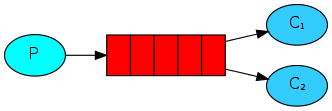
\includegraphics[scale=0.65]{cap_diseño/images/work-queues}
  \caption[Representación de las colas de trabajo. Ejemplo de comunicación asíncrona dirigida.]{Representación de las colas de trabajo. Ejemplo de comunicación comunicación asíncrona dirigida. \footnotemark }
  \label{fig:work-queues}
\end{figure}

\footnotetext{Imagen obtenida de: \url{https://www.rabbitmq.com/tutorials/tutorial-two-dotnet.html}}

Otra estrategia posible es \foreign{english}{publish-suscribe}: sirve para implementar comunicación \foreign{english}{multicast}. Se basa en el uso de \textbf{temas} o \textbf{\foreign{english}{topics}}: categorías de mensajes que pueden resultar de interés. Un servicio (el productor) envía un mensaje al \foreign{english}{broker}, indicando que pertenece a un tema determinado. El \foreign{english}{broker} recibe el mensaje y se encarga de reenviarlo a todos los servicios suscritos a este tema en concreto. \cite{rabbitmqPublishSubscribeDocumentation} En la figura \ref{fig:publish-subscribe} tenemos un ejemplo. El mensaje ''A'' llega a todos los servicios suscritos a al tema ''Topic''.

\textcolor{red}{Describir fanout}
\textcolor{red}{Describir exchanges}

\begin{figure}[htb]
  \centering
  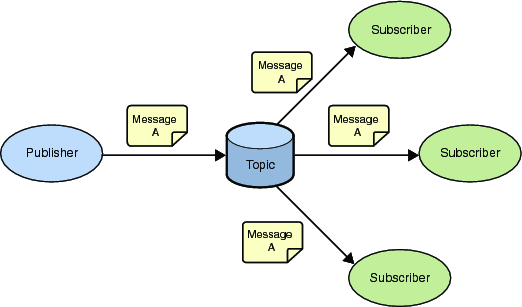
\includegraphics[scale=0.5]{cap_diseño/images/publish_subscribe}
  \caption[Estrategia \foreign{english}{publish/suscribe}: el \foreign{english}{broker} actúa como intermediario en la comunicación \foreign{english}{multicast}.]{Estrategia \foreign{english}{publish/suscribe}: el \foreign{english}{broker} actúa como intermediario en la comunicación \foreign{english}{multicast}. Imagen obtenida de \footnotemark.}
  \label{fig:publish-subscribe}
\end{figure}

\footnotetext{Java Messaging Service: \url{https://docs.oracle.com/cd/E19509-01/820-5892/ref_jms/index.html}}

La mayor ventaja de este estilo de comunicación es el \textbf{desacoplamiento} entre los servicios. \cite{korabUnderstandingMessageBrokers2017}
Ninguno de ellos necesita conocer detalles sobre cómo están desplegado los otros: su dirección, el número de instancias, si están activos en este momento, etc. Para enviar o recibir mensajes solo necesitan conocer su formato, las colas o temas y la dirección del \foreign{english}{broker}.

\begin{itemize}
  \item \textbf{Ventajas}:

  \begin{itemize}
    \item \textbf{Comunicación asíncrona}: El servicio no necesita quedarse a la espera de una respuesta del servidor. Puede procesar otras operaciones hasta que se le notifique del resultado, si lo hubiera.

    \item \textbf{Desacoplamiento de los servicios}: Ni los productores ni los consumidores necesitan conocer el origen o destino de sus mensajes. Solo su formato, las colas o temas y la dirección del \foreign{english}{broker}.

    \item \textbf{Envío garantizado de mensajes}: El \foreign{english}{broker} garantiza que el mensaje será entregado \emph{al menos} una vez al consumidor. Reintentará el reenvío hasta que se confirme su recepción.

  \end{itemize}

  \item \textbf{Desventajas}:

  \begin{itemize}
    \item \textbf{Requisitos de infraestructura}: Utilizar un \foreign{english}{broker} de mensajería puede incrementar la dificultad de nuestros despliegues. Este puede convertirse en un punto de fallo único. Para operar de forma fiable, estos sistemas requieren de replicación. \cite{newmanBuildingMicroservicesDesigning2021}

    \item \textbf{Envío garantizado de mensajes}: Para poder garantizar el envío de un mensaje, el \foreign{english}{broker} puede recurrir a reenviarlo. Debemos diseñar nuestros sistemas de forma que estos mensajes duplicados sean descartados si ya han sido procesados.
  \end{itemize}
\end{itemize}

En la tabla \ref{tab:comparativa-mecanismos-comunicacion} presentamos un resumen de esta comparativa:

\textcolor{red}{Añadir la cardinalidad de los conectores}

\begin{longtable}{|p{4.4cm} | c | c | c | c|}
  \hline
  & \textbf{RPC} & \textbf{REST} & \textbf{GraphQL} & \textbf{Broker mensajería} \\
  \hline
  \textbf{Tipo de comunicación entre componentes} & Dirigida & Dirigida & Dirigida & Dirigida y \foreign{english}{Multicast} \\
  \hline
  \textbf{Acoplamiento entre componentes} & Alto & Medio & Alto & Bajo \\
  \hline
  \textbf{Interoperabilidad} & Baja & Alta & Alta & Alta\footnotemark \\
  \hline
  \textbf{Comandos de lectura} & Sí & Sí & Sí & Sí\footnotemark \\
  \hline
  \textbf{Comandos de escritura} & Si & Sí & No & Sí \\
  \hline
  \textbf{Comunicación síncrona} & Sí & Sí & Sí & No \\
  \hline
  \textbf{Comunicación asíncrona} & No & Sí & No & Si \\
  \hline
  \caption{Comparativa de los mecanismos de comunicación.}
  \label{tab:comparativa-mecanismos-comunicacion}
\end{longtable}

\footnotetext{Depende de si tenemos control sobre los componentes que queremos integrar.}
\footnotetext{Aunque no es el mecanismo ideal para lecturas. Se recomienda que los mensajes sean ligeros. Los otros protocolos serían más adecuados.}

Ahora describiremos qué protocolo elegimos para cada mecanismo de comunicación.

\subsection{Peticiones síncronas}

Comenzamos investigando las peticiones síncronas. Tomemos por ejemplo la comunicación entre el servicio de monitorización (\foreign{english}{monitoring service}) y el servicio de conocimiento (\foreign{english}{knowledge servic}). Recordemos que el servicio de conocimiento almacena todas las propiedades de adaptación. El resto de servicios del nivel del bucle necesitan consultarlas y actualizarlas durante su funcionamiento. En la figura \ref{fig:monitor-knowledge-initial} representamos inicialmente ambos componentes y un conector, sin especificar de qué tipo será.

% TODO: Cambiar por imagen de componentes, que ofrezcan y requieran interfaces.
\begin{figure}[htb]
  \centering
  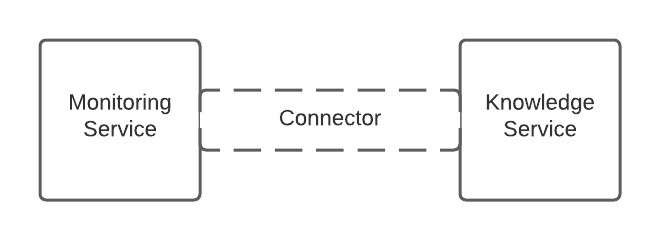
\includegraphics{cap_diseño/images/Monitor-Knowledge-Initial-Connector}
  \caption{Representación inicial de la comunicación entre el servicio de monitorización y el de conocimiento. El conector no indica su tipo todavía.}
  \label{fig:monitor-knowledge-initial}
\end{figure}

El siguiente paso es identificar qué interacciones debe existir entre ambos componentes. En este caso, el servicio de monitorización debe contactar con el servicio de conocimiento para leer y actualizar el valor de las propiedades. Por tanto, existen operaciones de lectura y escritura de los datos.

Entre las cuatro opciones de tipos de conector podemos descartar inmediatamente la opción de GraphQL. Se trata de un conector más orientado a las consultas de datos. En nuestro caso, necesitamos ejecutar también escrituras. Aunque podría ser interesante para consultas más avanzadas, utilizar dos protocolos de comunicación en paralelo aumentaría la complejidad de la arquitectura.

También descartamos el \foreign{english}{broker} de mensajería. Como requerimos de lecturas de datos, nos convenía más recurrir al resto de patrones. Para obtener propiedades del conocimiento, resultaba más sencillo de implementar mediante comunicación síncrona.

Finalmente, hay que tener en cuenta que una de nuestras prioridades es la \textbf{interoperabilidad}: esta API estará expuesta ''hacia fuera'', a una capa más externa. Por tanto, tendremos clientes que nos contactarán. Potencialmente, de terceros. Prima por tanto la compatibilidad. Descartamos entonces RPC, dado que nos acoplaría a una tecnología concreta y a APIs no estándares.

Nos terminamos decantando por el conector REST sobre HTTP. Implementamos ambas funciones mediante \foreign{english}{endpoints} HTTP. Su especificación se detalla a continuación en las tablas \ref{tab:especificacion-get-property} y \ref{tab:especificacion-put-property}.

\newsavebox\getpropertyrequestbox
\begin{lrbox}{\getpropertyrequestbox}
  \begin{minipage}[t]{1in}
    \begin{verbatim}
Request:
HTTP GET property/currentTemperature

Response: 200 Ok
{
  value: {
    "Value":16.79,
    "Unit": "Celsius",
    "ProbeId":"c02234d3-329c-4b4d-aee0-d220dc25276b",
    "DateTime":"2022-01-15T18:19:38.5231231Z"
  },
  lastModification: "2022-01-15T18:19:39.123213Z"
}
    \end{verbatim}
  \end{minipage}
\end{lrbox}

\begin{longtable}{|m{3.4cm}|p{2.5cm}|p{1cm}|p{3cm}|}
  \hline

  \textbf{Operación HTTP} & GET & \textbf{Ruta} & property/\{\emph{propertyName}\} \\
  \hline

  \textbf{Descripción} & \multicolumn{3}{|l|}{Devuelve el valor de la propiedad, si existe.} \\
  \hline

  \textbf{Parámetros} & \emph{propertyName} & \multicolumn{2}{|m{0.55\linewidth}|}{El nombre de la propiedad que deseamos obtener. Se lee a partir de la ruta de la petición.}\\
  \hline

  \multirow{3}*{\textbf{Respuestas posibles}}
        & \textbf{Código 200 (Ok)} & \multicolumn{2}{|m{0.55\linewidth}|}{La propiedad se ha encontrado. Incluye un \foreign{english}{payload} con el siguiente esquema:

        \begin{itemize}
          \item \foreign{english}{Value}: Valor de la propiedad serializado en JSON.
          \item \emph{LastModification}: Fecha y hora de la última modificación de esta propiedad.
        \end{itemize}}\\

        \cline{2-4}

        & \textbf{Código 400 (Bad request)} & \multicolumn{2}{|m{0.55\linewidth}|}{La petición está mal formada, no es acuerdo al contrato.}\\

        \cline{2-4}

        & \textbf{Código 404 (Not found)} & \multicolumn{2}{|m{0.55\linewidth}|}{No se ha encontrado ninguna propiedad con el nombre proporcionado.}\\
  \hline

  \textbf{Ejemplo} & \multicolumn{3}{|b{0.7\linewidth}|}{Petición para obtener la propiedad \emph{currentTemperature}:
  \usebox\getpropertyrequestbox} \\

  \hline

  \caption{Especificación de la operación para obtener una propiedad del servicio de conocimiento.}
  \label{tab:especificacion-get-property}
\end{longtable}

\newsavebox\putpropertyrequestbox
\begin{lrbox}{\putpropertyrequestbox}
  \begin{minipage}[t]{2in}
    \begin{verbatim}
Request:
HTTP PUT property/currentTemperature

{
  value: {
    "Value":16.79,
    "Unit": 1, // Celsius
    "ProbeId":"c02234d3-329c-4b4d-aee0-d220dc25276b",
    "DateTime":"2022-01-15T18:19:38.5231231Z"
  }
}

Response: 204 (No content)
        \end{verbatim}
  \end{minipage}
\end{lrbox}

\begin{longtable}{|m{3.4cm}|m{2.5cm}|b{1cm}|b{3cm}|}
  \hline

  \textbf{Operación HTTP} & PUT & \textbf{Ruta} & property/\{\emph{propertyName}\} \\
  \hline

  \textbf{Descripción} & \multicolumn{3}{|b{0.7\linewidth}|}{ Actualiza (o crea, si no existe) el valor de la propiedad con el nombre dado.} \\
  \hline

  \multirow{2}*{\textbf{Parámetros}}
        & \emph{propertyName} & \multicolumn{2}{|b{0.55\linewidth}|}{El nombre de la propiedad que deseamos crear o actualizar. Se lee a partir de la ruta de la petición.}\\

        \cline{2-4}

        & \emph{SetPropertyDTO} & \multicolumn{2}{|b{0.55\linewidth}|}{ Un DTO que contiene el valor a asignar en la propiedad serializado en JSON. El DTO se encuentra en el cuerpo de la petición.} \\
  \hline

  \multirow{2}*{\textbf{Respuestas posibles}}
        & \textbf{Código 204 (No content)} & \multicolumn{2}{|b{0.55\linewidth}|}{La propiedad se ha creado o actualizado correctamente. No incluye \emph{payload} en el cuerpo de la respuesta.}\\

        \cline{2-4}

        & \textbf{Código 400 (Bad request)} & \multicolumn{2}{|b{0.55\linewidth}|}{La petición está mal formada, no es acuerdo al contrato.}\\
  \hline

  \textbf{Ejemplo} & \multicolumn{3}{|b{0.7\linewidth}|}{Petición para actualizar la propiedad \emph{currentTemperature} con una medición de un termómetro:
  \usebox\putpropertyrequestbox} \\

  \hline

  \caption{Especificación de la operación para actualizar o crear una propiedad del servicio de conocimiento.}
  \label{tab:especificacion-put-property}
\end{longtable}

Una vez definida la interfaz que expondrá el servicio de conocimiento, nos quedaba definir cómo se invocaría desde el servicio de monitorización. ¿Implementamos las llamadas manualmente con un cliente HTTP? Aunque no sería muy complicado, tendríamos que mantenerlo manualmente cuando evolucione el sistema. Optamos entonces por una alternativa: generar clientes a partir del estándar OpenAPI.

\subsubsection{Open API}
\label{chap:OpenAPI}

\begin{wrapfigure}{r}{0.3\linewidth}
  \vspace{5pt}
  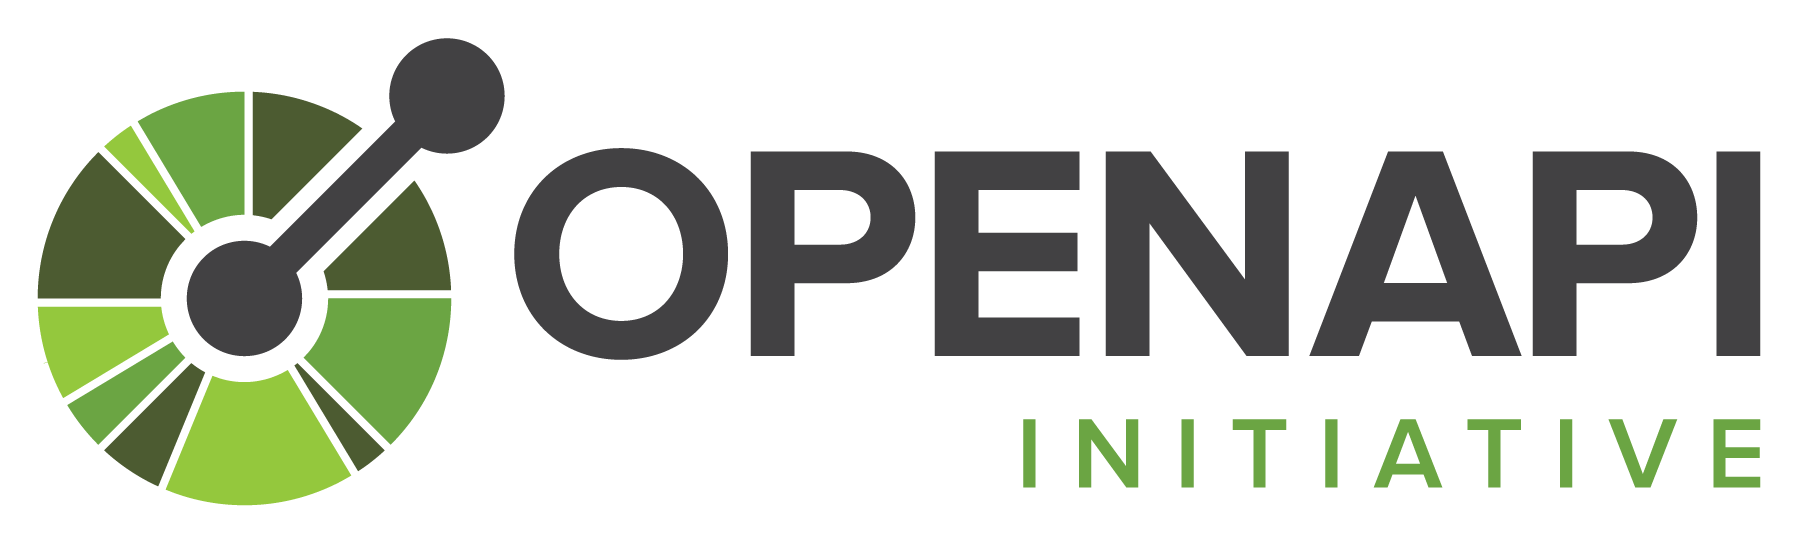
\includegraphics[scale=0.32]{cap_diseño/images/openapi-logo}
  \centering
  \vspace{5pt}
\end{wrapfigure}

OpenAPI\footnote{Página oficial: \url{https://www.openapis.org/}} es un lenguaje estándar para describir APIs RESTful. Nos permite describir de forma estructurada las operaciones que ofrece un servicio manteniéndose agnóstico a su implementación. Esta descripción ayuda tanto a humanos como a computadoras a descubrir y utilizar las funcionalidades de la API. La OpenAPI Initiative (OAI) dirige el proyecto bajo el manto de la \emph{Linux Foundation}.

Un documento OpenAPI describe el funcionamiento de la API y el conjunto de recursos que la componen. Describe las operaciones HTTP que podemos ejecutar sobre estos recursos, incluyendo las estructuras de datos que recibe o envía y los códigos de respuesta. Estos códigos indican al cliente el resultado de la ejecución de la operación. \cite{openapi_initiativeOpenAPISpecificationV3} Más adelante mostraremos un ejemplo, con el \textcolor{red}{fragmento} \ref{ls:openapi-get}.

La especificación puede escribirse manualmente o puede generarse a partir de una implementación existente. Así, podemos desarrollar nuestro servicio en un determinado lenguaje y obtener su descripción en OpenAPI. Además, podemos aprovecharla en varios ámbitos del desarrollo gracias a la variedad de herramientas existentes: generación de documentación, generación de casos de prueba, identificar cambios incompatibles, etc. \cite{westerveldChapterOpenAPIAPI2021}

Uno de los casos de uso más interesantes es la generación de código a partir de la definición. Existen una serie de librerías\footnote{\url{https://github.com/OpenAPITools/openapi-generator}} capaces de generar clientes o servidores conforme a la especificación. Ofrecen soporte a una gran variedad de lenguajes: Java, C\#, JavaScript\dots En el caso del cliente, actúa como un proxy que nos abstrae de la lógica de comunicación con el servidor. Similar a lo descrito en el apartado de RPC.

Para el desarrollo de este trabajo, nos interesaba especialmente debido a las diferencias tecnológicas existentes: el bucle MAPE-K original estaba desarrollado en Java, pero el prototipo se desarrolló con el lenguaje C\# usando el \foreign{english}{framework} ASP.NET Core. Se tomó esta decisión para reducir el tiempo de aprendizaje y centrar los esfuerzos en la definición de la arquitectura del sistema.

Gracias a la generación de código, se podría obtener la especificación del prototipo y generar los clientes o servidores en cualquier lenguaje soportado. Java incluido. El bucle MAPE-K original después podría ser refactorizado usando este código autogenerado.

A continuación explicaremos cómo utilizamos OpenAPI. Para ello, continuaremos con el ejemplo del servicio de conocimiento que hemos descrito a lo largo de esta sección. Nos centraremos en la implementación de la operación para obtener una propiedad del conocimiento, descrita en la tabla \ref{tab:especificacion-get-property}.

En el \textcolor{red}{fragmento} \ref{ls:csharp-get} podemos observar que se trata de un método C\# llamado \emph{GetProperty}. Su implementación es sencilla: busca en un diccionario la propiedad cuyo nombre se le pasa por parámetro. Si la encuentra, devuelve su valor con un código 200 OK. En caso contrario, devuelve un código de error que describe el motivo (formato de la petición incorrecto o no se ha encontrado la propiedad).

Aparte de la implementación, podemos comprobar que el método cuenta con una serie de comentarios (líneas 1-8) y atributos (10-12). Esta documentación describe qué hace el método, sus entradas y posibles respuestas. OpenAPI es capaz de utilizarlos para generar una especificación más completa. Por tanto, resulta muy recomendable incluirlos.

\begin{lstlisting}[language={[Sharp]C},caption={Implementación del método GetProperty decorado para generar la especificación OpenAPI.},captionpos=b, label=ls:csharp-get]
/// <summary>
///    Gets a property given its name.
/// </summary>
/// <param name="propertyName"> The name of the property to find. </param>
/// <returns> An IActionResult with result of the query. </returns>
/// <response code="200"> The property was found. Returns the value of the property. </response>
/// <response code="404"> The property was not found. </response>
/// <response code="400"> There was an error with the provided arguments. </response>
[HttpGet("{propertyName}")]
[ProducesResponseType(typeof(PropertyDTO), StatusCodes.Status200OK)]
[ProducesResponseType(StatusCodes.Status404NotFound)]
[ProducesResponseType(StatusCodes.Status400BadRequest)]
public IActionResult GetProperty([FromRoute]string propertyName)
{
    if (string.IsNullOrEmpty(propertyName))
    {
        return BadRequest();
    }

    bool foundProperty = properties.TryGetValue(propertyName, out PropertyDTO property);

    if (!foundProperty)
    {
        return NotFound();
    }

    return Ok(property);
}
\end{lstlisting}

Haciendo uso de las librerías de OpenAPI, generamos la especificación a partir del servicio de conocimiento. En el \textcolor{red}{fragmento} \ref{ls:openapi-get}, podemos ver cómo se describe la operación en este estándar:

\begin{lstlisting}[language=python,caption={Especificación OpenAPI del método para obtener una propiedad del conocimiento (\lstinline{GetProperty}).},captionpos=b, label=ls:openapi-get]
"paths": {
  "/Property/{propertyName}": {
    "get": {
      "tags": [
        "Property"
      ],
      "summary": "Gets a property given its name.",
      "parameters": [
        {
          "name": "propertyName",
          "in": "path",
          "description": "The name of the property to find.",
          "required": true,
          "schema": {
            "type": "string"
          }
        }
      ],
      "responses": {
        "200": {
          "description": "The property was found. Returns the value of the property.",
          "content": {
            "application/json": {
              "schema": {
                "$ref": "#/components/schemas/PropertyDTO"
              }
            }
          }
        },
        "404": {
          "description": "The property was not found.",
        },
        "400": {
          "description": "There was an error with the provided arguments.",
        }
      }
    }
  }
\end{lstlisting}

Podemos apreciar que en la ruta \emph{/Property/\{propertyName\}} está disponible una operación de tipo \emph{GET}. Esta acepta determinados parámetros y describe unas posibles respuestas. También aparece una referencia a otro esquema (línea 25), que representa la estructura de la respuesta en ese caso concreto. También aparecen los comentarios opcionales que indicamos en el \textcolor{red}{fragmento} \ref{ls:csharp-get}. Encontramos grandes similitudes con la especificación presentada en la tabla \ref{tab:especificacion-get-property}.

%% TODO: ¿Eliminar?
\textcolor{red}{Los convenios de los generadores de código de OpenAPI pueden no ser de nuestro agrado. Por ejemplo, pueden resultar muy verbosos o puede resultar muy pesado trabajar con DTOs directamente. Por suerte, tenemos varias alternativas para solucionarlo: Modificar las plantillas de generación de código. Al ser de código abierto, podríamos modificar las existentes o crear nuestras propias plantillas con nuestros propios convenios.}

\textcolor{red}{Otra opción, más fácil de implementar, es desarrollar código por encima del API Client generado. Es el caso del servicio de Análisis. Como trabajar con DTOs directamente se hacía muy pesado (fragmento \ref{ls:analysis-api-client-original}), optamos por implementar un \foreign{english}{builder} de peticiones. Esto nos permitia configurar la petición de una forma más descriptiva para el usuario (fragmento \ref{ls:analysis-api-cliente-request-builder}):}

\begin{lstlisting}[language={[Sharp]C},caption={Implementación de petición original. Trabajar con DTOs era muy verboso.},captionpos=b, label=ls:analysis-api-client-original]
var changeRequests = new List<ServiceConfigurationDTO>
{
  new()
  {
    ServiceName = ClimatisationAirConditionerConstants.AppName,
    IsDeployed = true,
    ConfigurationProperties = new List<ConfigurationProperty>()
    {
      new()
      {
          Name = ClimatisationAirConditionerConstants.Configuration.Mode,
          Value = AirConditioningMode.Cooling.ToString(),
      },
    },
  },
};

var symptoms = new List<SymptomDTO> { new(SymptomName, "true") };

var systemConfigurationChangeRequest = new SystemConfigurationChangeRequestDTO()
{
  ServiceConfiguration = changeRequests,
  Symptoms = symptoms,
  Timestamp = DateTime.UtcNow,
};

await _systemApi.SystemRequestChangePostAsync(
  systemConfigurationChangeRequest,
  CancellationToken.None);
\end{lstlisting}


\begin{lstlisting}[language={[Sharp]C},caption={Implementación de la misma petición siguiendo el patrón \emph{builder}.},captionpos=b, label=ls:analysis-api-cliente-request-builder]
await _systemService.RequestChangeAsync(changeRequest =>
{
  changeRequest
    .ForSymptom(TemperatureGreaterThanHotThreshold)
    .WithService(ClimatisationAirConditionerConstants.AppName, service =>
    {
      service.MustBePresent()
        .WithParameter(
          ClimatisationAirConditionerConstants.Configuration.Mode,
          AirConditioningMode.Cooling.ToString());
    });
});
\end{lstlisting}

Para terminar, mostramos la estructura del conector que emplearemos para implementar las peticiones aparece en la figura \ref{fig:monitor-knowledge-connector-architecture}. La figura muestra como el servicio de monitorización contacta al de conocimiento para asignarle un valor a la propiedad \emph{Temp}.

El conector, delimitado por una línea discontinua roja, está compuesto por dos elementos: una API REST y un cliente. Los otros dos grupos de elementos representan los procesos de los servicios de monitorización y conocimiento. El servicio de monitorización se comunica a con la API través del API Client, que está en su proceso actuando como \emph{proxy}.

%%% TODO: Actualizar la imagen para que aparezca PUT en vez de POST.
%%% TODO: ¿Darle la vuelta a los servicios? Monitor arriba y Knowledge abajo.
\begin{figure}[htb]
  \centering
  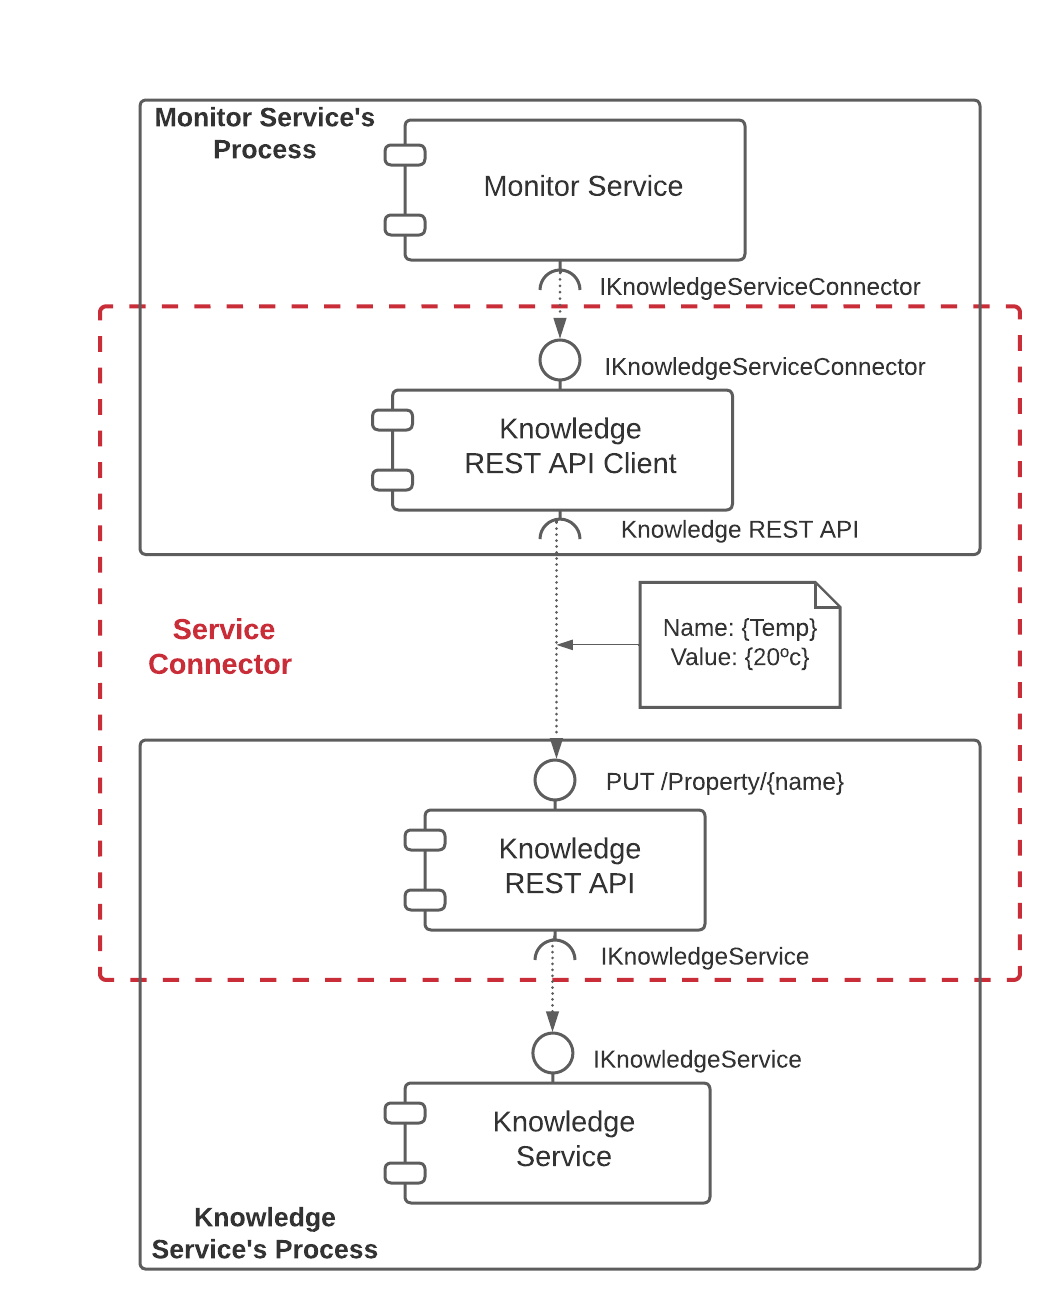
\includegraphics[scale=0.64]{cap_diseño/images/Monitor-Knowledge-Connector}
  \caption{Diseño del conector usando implementación Cliente - Servidor}
  \label{fig:monitor-knowledge-connector-architecture}
\end{figure}

\subsection{Notificaciones}
\label{sec:notificaciones}

El siguiente mecanismo de comunicación que tratamos fueron las notificaciones. Recordemos que esta comunicación consiste en transmitir mensajes desde un servicio a todos los que se pertenecen a la capa superior. Es una comunicación de tipo \emph{multicast}. No va dirigida a ningún servicio concreto. Potencialmente, todos podrían recibir el mensaje y decidir si procesarlo o no.

Para estudiarla, tomamos como ejemplo la comunicación entre el servicio de conocimiento y los servicios en el nivel del bucle. Cada vez que se modifique una propiedad de adaptación o una clave de configuración, emitirá un evento a la capa superior. Así, por ejemplo, el servicio de análisis sabrá que debe reevaluar las reglas de adaptación.

Buscando el tipo de conector adecuado, empezamos descartando GraphQL. Es un protocolo basado en lecturas. Como el objetivo es enviar información a otros servicios, no nos sirve. Respecto a RPC y REST, tampoco cumplían nuestras necesidades. Tenemos el requisito de bajo acoplamiento contra los servicios de la capa superior. Estos protocolos requerirían de conocer la dirección de todos los servicios para poder contactarlos. O, en su defecto, requeririamos de implementar un intermediario que los tenga registrados.

Por tanto, optamos por implementarlo usando un \emph{broker} de mensajería. Concretamente, siguiendo el patrón \emph{publish}-\emph{subscribe}. El servicio de conocimiento publicará el evento a través del \emph{broker} en un \foreign{english}{exchange} determinado. Este evento tendrá como \emph{topic} o tema asociado el nombre de la propiedad. Todos los servicios interesados deberán suscribirse a este. El \emph{broker} añadirá el mensaje en la cola de cada uno de los suscriptores. Así podrán procesarlo cuando puedan, de forma asíncrona.

En la tabla \ref{tab:especificacion-property-changed-integrationevent} mostramos la especificación del evento. Podemos apreciar que el mensaje enviado incluye la información mínima indispensable: el nombre de la propiedad que ha cambiado. Tomamos esta decisión porque se trata de una comunicación asíncrona. Desde que se emite el evento hasta que se procesa su valor puede haber cambiado. De esta forma obligamos a las reglas a solicitar el valor de la propiedad en el momento en que se evalúen. Entonces siempre se ejecutaran con la información actualizada.

\newsavebox\propertychangedeventbox
\begin{lrbox}{\propertychangedeventbox}
  \begin{minipage}[t]{2in}
    \begin{verbatim}
{
  "PropertyName":"Temperature"
}
        \end{verbatim}
  \end{minipage}
\end{lrbox}

\begin{table}[htb]
  \centering

  \begin{tabular}{|m{2.3cm}|p{2.5cm}|p{2.6cm}|b{1.5cm}|b{1.5cm}|}
      \hline

      \textbf{Evento} & \multicolumn{2}{|b{0.35\linewidth}|}{\emph{PropertyChangedIntegrationEvent }} & \textbf{\emph{Exchange}} & \emph{AdaptionLoop.Knowledge}  \\
      \hline

      \textbf{Descripción} & \multicolumn{4}{|b{0.6\linewidth}|}{Evento de integración que notifica sobre el cambio de una propiedad adaptación.} \\
      \hline

      \textbf{Propiedades}
            & \emph{propertyName} & \multicolumn{3}{|b{0.6\linewidth}|}{Nombre de la propiedad que ha cambiado.} \\
      \hline

      \textbf{Ejemplo} & \multicolumn{4}{|b{0.7\linewidth}|}{Evento que notifica del cambio de la propiedad \emph{Temperature}:\linebreak
      \usebox\propertychangedeventbox} \\

      \hline
  \end{tabular}

  \caption{Especificación del evento que notifica sobre el cambio de una propiedad del conocimiento.}
  \label{tab:especificacion-property-changed-integrationevent}
\end{table}

\subsubsection{AsyncAPI}

Para describir el evento, investigamos si existía algún estándar equivalente a OpenAPI. Y así es, se llama AsyncAPI\footnote{Página oficial: \url{https://www.asyncapi.com/}}. Por desgracia, se encuentra en fases tempranas de su desarrollo. No ha alcanzado todavía el grado de implantación que tiene su homólogo. Por ejemplo, no cuenta un catálogo muy amplio de generadores de código. Tampoco podemos extraer la especificación a partir de una implementación existente.

Aun así, lo emplearemos para describir manualmente nuestros eventos en un formato estándar. En el fragmento \ref{ls:asyncapi-propertychanged-integrationevent} presentamos la especificación del mensaje de la tabla \ref{tab:especificacion-property-changed-integrationevent}. Podemos apreciar similitudes con la especificación OpenAPI (por ejemplo, en el fragmento \ref{ls:openapi-get}). Figura la estructura del mensaje y su documentación. La mayor diferencia es la mención del canal (el \foreign{english}{exchange}  en nuestro caso) y el método (\foreign{english}{subscribe}). Esto indica que los consumidores podrán suscribirse a este evento a partir de este canal.

% TODO: Pintar bien los YAML.
\begin{lstlisting}[language={C++},caption={Ejemplo del evento de integración \emph{builder}.},captionpos=b, label=ls:asyncapi-propertychanged-integrationevent]
asyncapi: 2.4.0
info:
  title: Knowledge Service
  version: 1.0.0
  description: This service contains all the adaptation properties to inform the different stages of the loop.
channels:
  AdaptionLoop.Knowledge:
    subscribe:
      message:
        $ref: '#/components/messages/PropertyChangedIntegrationEvent'
components:
  messages:
    PropertyChangedIntegrationEvent:
      description: >-
        Integration event notifying about a change in an adaption property.
      payload:
        type: object
        properties:
          propertyName:
            type: string
            description: The name of the property that changed
\end{lstlisting}

\subsubsection{Diseño del conector}

Para implementar este patrón, nuestro conector estará compuesto por tres elementos: un publicador, el \foreign{english}{broker} y un consumidor. Pongamos por ejemplo que el servicio de conocimiento recibe una petición para actualizar una propiedad. Si esta actualización se lleva a cabo, deberá propagar el evento a través del publicador. Este enviará el mensaje al \foreign{english}{broker} a un \foreign{english}{exchange} determinado.

El \foreign{english}{broker}, que conoce todos los suscriptores, lo añadirá en la cola de mensajería de cada uno de ellos. Sus consumidores, desplegados en cada servicio suscriptor, serán notificados del nuevo mensaje. Los procesarán en cuanto puedan. En la \textcolor{red}{figura X} mostramos la estructura de este nuevo conector.

\textcolor{red}{TODO: Imagen del conector. Similar a \ref{fig:monitor-knowledge-connector-architecture}}

\subsection{Peticiones asíncronas}

El mecanismo de comunicación restante son las \textbf{peticiones asíncronas}. Se trata de peticiones de trabajo que un microservicio le envía a otro distinto. Ambos deberán encontrarse mismo nivel de la jerarquía. Como comentamos, tenemos dos casos en nuestra arquitectura que requieren de este patrón: la comunicación entre el módulo de análisis y el planificador; y aquella entre el planificador y el ejecutor. Nos centraremos en el primero.

Cuando se evalúan las reglas de adaptación, si alguna de ellas se ejecuta, propone un cambio en la configuración del sistema. Como estos servicios están en una capa superior a la del bucle, se lo transmiten al servicio de análisis mediante una petición síncrona. El módulo de análisis recibirá esta propuesta y la enviará al planificador mediante una petición asíncrona. Podríamos haberla enviado directamente directamente al servicio de planificación, pero preferimos que no se acoplen a un servicio adicional.

A la hora de escoger el mecanismo de comunicación, el razonamiento fue muy similar al empleado en las notificaciones. Optamos por implementarlas usando un \foreign{english}{broker} de mensajería, pero siguiendo el patrón de colas de trabajo. Los \foreign{english}{workers} cuentan con una cola de mensajería específica para las peticiones de trabajo. El publicador la conoce y, a través del  \foreign{english}{broker}, envía los mensajes allí. El consumidor los irá recuperando y procesando en cuando esté disponible.

En la tabla \ref{tab:especificacion-system-configuration-change-request-box} presentamos la especificación de la petición asíncrona para solicitar un cambio de configuración de sistema. Vemos que es muy similar a \ref{tab:especificacion-property-changed-integrationevent}. La principal diferencia es que esta incluye mucha más información que el evento. Esto es debido a que tiene más en común con una petición síncrona. El consumidor recibirá todos los parámetros que necesita para ejecutar la petición. Aun así, en el momento de ejecución, deberá verificar que algunos de estos parámetros no hayan cambiado.

\newsavebox\systemconfigurationchangerequestbox
\begin{lrbox}{\systemconfigurationchangerequestbox}
  \begin{minipage}[t]{2in}
    \begin{verbatim}
{
  "Timestamp": "2022-06-19T16:38:30.6092751Z",
  "Symptoms":[
    {
      "Name": "temperature-lesser-than-cold-threshold",
      "Value": "true"
    }
  ],
  "ConfigurationRequests":  [
    {
      "ServiceName": "Climatisation.AirConditioner.Service",
      "IsDeployed": true,
      "ConfigurationProperties": [
        {
          "Name": "Mode",
          "Value": "Heating"
        }
      ],
      "Bindings": []
    }
  ]
}
        \end{verbatim}
  \end{minipage}
\end{lrbox}

\begin{longtable}{|m{2cm}|m{2.3cm}|m{10cm}|b{0.85cm}|b{2.75cm}|}
  \hline

  \textbf{Nombre} & \multicolumn{2}{|b{0.37\linewidth}|}{\emph{SystemConfigurationChangeRequest}} & \textbf{Cola} & \emph{AdaptionLoop.Planification.Requests}  \\
  \hline

  \textbf{Descripción} & \multicolumn{4}{|b{0.82\linewidth}|}{Petición que representa una propuesta de cambio de la configuración del sistema.} \\
  \hline

  \textbf{Propiedades}
    & \emph{Timestamp} & \multicolumn{3}{|m{0.67\linewidth}|}{Fecha y hora de la petición de cambio.} \\
    \cline{2-5}
    & \emph{Symptoms} & \multicolumn{3}{|m{0.67\linewidth}|}{Colección de síntomas que la han desencadenado.} \\
    \cline{2-5}
    & \emph{Configuration Requests} & \multicolumn{3}{|m{0.67\linewidth}|}{Colección peticiones de configuración de la propuesta de cambio.

    Cada una de estas está compuesta por:
    \begin{itemize}
      \item \textbf{\emph{ServiceName}}: Identificador del servicio cuya configuración queremos cambiar.
      \item \textbf{\emph{IsDeployed}}: Indica si el servicio debe estar desplegado o no en la siguiente configuración.
      \item \textbf{\emph{Bindings}}: Colección de conexiones que indican a qué otros servicios debe estar conectado (o no) en la siguiente configuración.
      \item \textbf{\emph{ConfigurationProperties}}: Colección de pares clave-valor que representan valores de su configuración que queremos actualizar.
    \end{itemize}} \\
  \hline

  \textbf{Ejemplo} & \multicolumn{4}{|b{0.82\linewidth}|}{Solicitud de cambio del modo de un aire acondicionado a modo calefacción (\emph{heating}). Los síntomas indican que fue desencadenada porque la temperatura era menor que un umbral determinado:\linebreak
  \usebox\systemconfigurationchangerequestbox} \\

  \hline

  \caption{Especificación de las peticiones de cambio de configuración del sistema.}
  \label{tab:especificacion-system-configuration-change-request-box}
\end{longtable}

Respecto a la especificación con AsyncAPI, las peticiones asíncronas no están soportadas todavía. A fecha de la redacción, el grupo se encuentra estudiando cómo implementarlas. \footnotetext{Discusión disponible en: \url{https://github.com/asyncapi/spec/pull/594}}. Su inclusión está propuesta para la versión 3.0.0 de la especificación. Como mencionamos anteriormente, el estándar todavía se encuentra en fases iniciales de su desarrollo.

\subsubsection{Diseño del conector}

En cuanto a sus componentes, el conector seguiría la siguiente arquitectura: \textcolor{red}{dibujo de arquitectura. La arquitectura del conector es muy similar a la de las notificaciones: un publicador, un broker y un consumidor.}

\section{Diseño final}

Añadir diagrama con el diseño final, mostrando el diseño de los componentes con todos los conectores.
